\documentclass[11pt, twocolumn]{article}

% GRAPHICS
\usepackage{float}
\usepackage{graphicx}
\usepackage{subcaption}

% HYPERLINKS
\usepackage{hyperref}

% DOCUMENT PADDING AND MARGINS
\usepackage{titlesec}
\usepackage[margin=0.8in]{geometry}
%\setlength{\parskip}{\baselineskip}%
%\setlength{\parindent}{0pt}
\titlespacing*{\section}{0pt}{2ex}{0ex}
\titlespacing*{\subsection}{0pt}{2ex}{0ex}
\titlespacing*{\subsubsection}{0pt}{2ex}{0ex}

% COMMENTING
\usepackage{comment}

% MATH FONTS
\usepackage{amsmath}


\begin{document}

% TITLE
\title{Autonomous Quadrotor Landing on a Moving Platform}
\author{Stan Brown \& Chris Choi}
\date{}
\maketitle

\section{Introduction}
Over the years there has been been a growing interest in autonomous landing of quadrotors as landing is often one of the most dangerous and risk prone parts of flight. There are now several commercial and research based implementations of autonomous landing with the DJI Phantom and Pixhawk flight controller both being capable of automatic landing using a series of sensors and control algorithms. However there does not yet seem to be a reliable method of landing a quadrotor on either a moving platform or in cases where there is relatively large cross wind disturbance. 

In recent years there have been at least least 5 academic publications on the topic \cite{Lee2012, Kim2014, Voos2010, Friis2009, Ling2014, Herisse2012} that approach the problem from a variaty of angles. Overall none of these approachs have solved the issue and most only work on very slow moving platforms with little or no wind disturbances. One of the most challenging with autonomous precision landing is the difficulty of obtaining a reliable estimate of the landing target relative to the quadrotor, the landing target can often go out of the camera's field of view causing the quadrotor to lose track of the target, other vision based artifacts that include lighting, lens distortion, color, etc.

The autonomous landing problem can be thought of as a set of three separate control problems or stages. First the quadrotor must detect the relative position and velocity of the landing target using either GPS of visual methods. Next the quadrotor must determine a rendezvous location with the landing target and plan the required flight trajectory. Once the quad has rendezvoused a final landing trajectory must be calculated between quadrotor and the landing pad. 

In this project we focus developing a set of controllers that produce the final landing trajectory and using a fiducial marker called an AprilTag \textbf{\textit{CITE APRILTAGS}} to provide the estimated state of the quadrotor relative to the landing pad. 

\section{Related Work} \textbf{(Needs love but might also just be cut.) }

For perception existing solutions use a variety of simple to complex techniques. In \cite{Kim2014} a basic color threshold technique was to identify the landing target, while \cite{Herisse2012} used optical flow in images captured on board the quadrotor to obtain necessary relative information for control. 

A comparison between a PID and Linear Quadratic Control (LQC) was explored in \cite{Friis2009}. However the authors admit, even though LQC performed slightly better than the PID controller the difference was minor and may be attributed to the additional time spent tuning the LQC. In \cite{Herisse2012} a PID controller was developed to land on a oscillating platform in the vertical direction with no lateral movement. While interesting, the solution took over 1 minute to transition from hovering over the landing pad to landing. Additionally the experiments did not seem to account for pitch or roll of the platform.  

\section{Methodology}
The majority of effort in this project so far can be separated into two individual but complementary pieces. First, a significant effort effort was spent on ensuring the quadrotor's state was updated a a rate of at least 20 $Hz$. Next, using the information in the state  a set of PID controllers were developed that along with a state machine monitors the current relative position of the quadrotor and either initiates a landing procedure or attempts to minimize the relative displacement and velocity between the quadrotor and the landing pad in the horizontal plane. 

\subsection{Measurement and State Estimation using AprilTags}
One of the major challenges when using AprilTags on a robot that has limited computational power, such as a quadrotor, is the rate at which the AprilTag library can compute the state. This problem is exacerbated when using larger image sizes as the computational time of the AprilTag software appears to grow at least exponentially as shown in (add a figure here). This problem was also noted in the work of \cite{Ling2014} and he addressed the issue by reducing the brightness of the image so that majority of the image is black except for the AprilTag. An example of this implementation is shown in figure (Kevins image). This allowed Ling \cite{Lee2012} to calculate states at a rate of approximatly 10 - 15 fps but it came at the cost of requiring the brightness parameters to be set ahead of time and also removed a lot of the robustification that is provided in the standard AprilTag library.

In this work, the slow rate of state estimation was addressed using a novel method where the image size and calibration parameters are set depending on the current distance between the quadrotors position relative to the landing pad. 

\subsubsection{Adaptive Image Preprocessing}

As discussed previously, the low rate of the AprilTag library when processing images of 640 by 480 pixels results in an update rate of approximately 3 to 5 fps on a Snapdragon 8 core processor, which is to low to be used effectively in a PID control loop. Building on the work of Ling, who noted that higher update rates were possible using AprilTags when the majority of the image is filled with black pixels, a set of image preprocessing methods were developed to maximize the update rate of the AprilTag library. 

\subsubsection{Adaptive Image Windowing}

If one assumes that the quadrotor does not move to fast, there is relativity low rotation between image captures, and that the image update rate is quite fast (60 fps in this implementation), then the location the AprilTag in the following image can be estimated based off of the location it was last observed in the previous image. Therefore whenever an AprilTag is measured in an image, a bounding box around the AprilTag is calculated and then used in the following image to black out the protions of the image where the AprilTag is unlikely to be. An example of this implementation is highlighted in Figure (Adptive windowing).


While the adaptive windowing procedure works well for when the AprilTag observed at a distance, where they do not take up a significant portion of the image, it begins to fail when the quadrotor approach the landing pad as the observed size of AprilTag begins to become larger and larger in the  image. This leads to the processing time of the AprilTags to increase as the quadrotor gets closer, which is a major issue as in these cases a higher update rate is actually required. In cases where the AprilTag is not observed in the expected location (bounding box), the size of the bounding box is set to the size of the image and the entire image is processed. 

\subsubsection{AprilTag Inception}
 In order to be used for landing, the AprilTag attached to the landing pad must be relatively larger so that it can be detected from a distance of at least 15 meters which from our experience means the AprilTag must be at least 50 cm by 50 cm in size. The large size of the AprilTag becomes a major issue during the final portion of the landing procedure as the AprilTag image will both appear quite large in the captured image which causes to the Adaptive Windowing Procedure outlined above to become ineffective. Furthermore close proximity to the AprilTag also grealy increases the chance that a portion of the AprilTag will be located outside of the captured image, causing no state estimation to be provided at the critical stages of landing. 
 
To address both the decreasing state update rate as a function of proximity and reduce the probablity of losing site of the AprilTag during landing a secondary AprilTag is embedded in the larger AprilTag. This secondary AprilTag is assigned different family id, and is placed in the center of a primary AprilTag. Whenever the secondary AprilTag is captured in the image, the adaptive windowing method is set to track only the secondary AprilTag rather than the larger one, which reduces the portion of the image that must be processed in with each image capture. An example of this procedure is highlighted in Figure \ref{fig:apriltagInception}.

\begin{figure}[H]
	\centering
	\begin{subfigure}[b]{0.45\linewidth}
		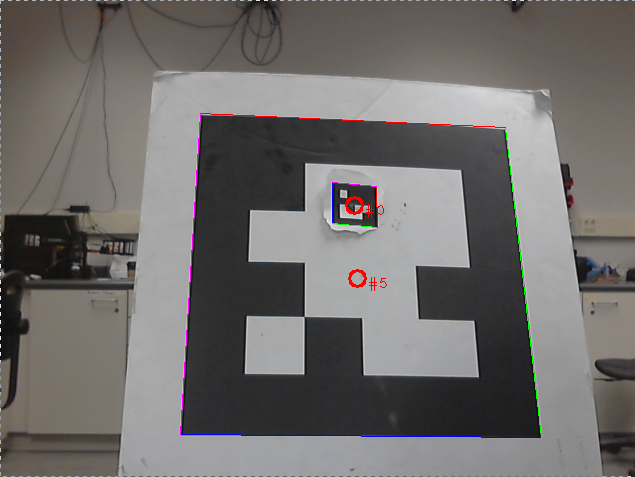
\includegraphics[width=\textwidth]{images/apriltags_1.png}
		\caption{2 Apriltags Detected}
	\end{subfigure}
	\begin{subfigure}[b]{0.45\linewidth}
		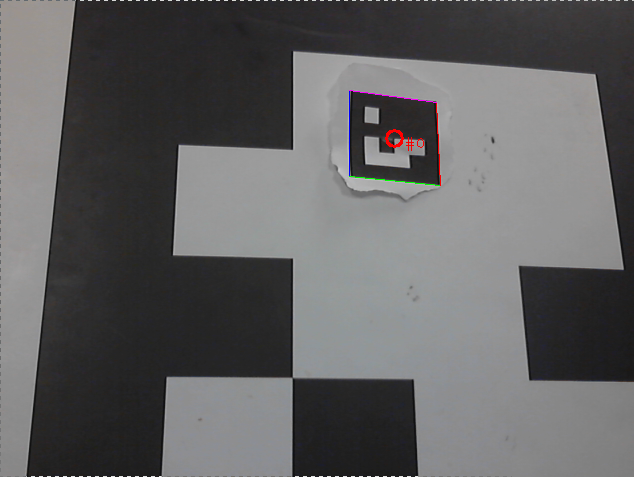
\includegraphics[width=\textwidth]{images/apriltags_3.png}
		\caption{1 Apriltag Detected }
	\end{subfigure}
	\caption{Apriltag Inception - To mitigate the FOV problem assocaited with }
	\label{fig:apriltagInception}
\end{figure}

\subsubsection{Adaptive Image Down-sampling}
It was also noted that the image could be greatly down sampled as well if the quadrotor approaches the landing pad as not as many pixels are required to calculated the location and state of the AprilTag in the image. Therefore 3 image sampling sizes were also introduced into the code which sub-sample the image to 160 by 140 pixels and 320 by 280 (half and quarter resolution) when the distance between the camera and the AprilTag is less than 1.5 and 3 meters respectively. If the camera is further than 3 meters from the AprilTag the native resolution of 640 by 480 is used. This change only affected the image processing time when the quadrotor is within 3 meters of the quad and has the desired effect of increasing the rate of AprilTag process.

In order to use this down sampling effectively without corrupting the AprilTag estimations, 3 camera calibration files were also computed at the normal, half and quarter camera resolutions. The calibration file passed to the AprilTag library during the state estimation procedure is selected based on what the current camera resolution is set at. 

\subsection{Controller and State Monitoring}
In this project it is assumed that the quadrotor has successfully rendezvoused with the target vehicle and at all points in time has a clear view through the camera image of the landing target located on the target vehicle. The first step of performing  autonomous landing is to position the quadrotor above the landing target such that the displacements in the x and y directions in the horizontal plane normal to the landing surface are near zero while simultaneously matching speed with the target vehicle. Next, while maintaining the near zero displacements in the x and y directions, the quadrotor must begin to descend at a safe rate such that the vertical distance between the quadrotor and the landing target is reduced until landing is achieved. Ideally the quadrotor will descend more rapidly when the vertical displacement between the qaudrotor and target is large, slowing down just before it hits the target in order to minimize time and energy requirements of the landing Vancouver. 

In order to achieve the described behaviour, a set of 3 of PID controllers are developed, one for the x, y and z directions respectively. During all stages of landing the x and y PID controllers work to minimize the displacement between the target and the qaudrotor which also has the side effect of maintaining the velocity relative to the target. During the approach the PIDz controller attempts to maintain a safe approach altitude such that the target does not go out of view during stage one. Once a these hold displacement value in x and y is achieve the $PID_z$ controller is set a set of commands that smoothly move the quadrotor to a landing position. 

The PIDx and PIDy are designed such that thier output is mapped to attitude commands in the pitch and roll relative to the quadrotor frame as outlined in Equations \ref{PIDx}, \ref{PIDy}, \ref{PIDz} . The commanded throttle is also adjusted to account for the commanded roll and pitch using Equation \ref{Adjusted Throttle} to better maintain altitude when $\phi_t$ and $\psi_t$ are non-zero. 

\begin{equation}
\label{PIDx}
	\psi_t = cos(\theta) \left( K_p e_x + K_i \sum_{t=0}^{t} \dot{e_x}_{,t} dt + K_d \dot{e_x}_{,t}) \right)
\end{equation}

\begin{equation}
\label{PIDy}
	\phi_t = sin(\theta) \left( K_p e_y + K_i \sum_{t=0}^{t} \dot{e_y}_{,t} dt + K_d \dot{e_y}_{,t} \right)
\end{equation}

\begin{equation}
\label{PIDz}
	Thrust_z = K_p e_z + K_i \sum_{t=0}^{t} \dot{e_z}_{,t} dt + K_d \dot{e_z}_{,t} 
\end{equation}

\begin{equation}
\label{Adjusted Throttle}
	AdjustedThrust = \frac{Thrust_z}{cos(\phi_t) cos(\psi_t)}
\end{equation}


\section{Experimental Hardware}
The quadrotor used in this experiment assembled from a DJI F450 quadrotor frame, 4 Emax 2213-935KV motors with complementary DJI E310 420S 20A electronic speed controllers. The flight controller selected for the project was a Pixhawk v2.4 running the PX4 firmware stack. An Odroid XU4 was selected as the onboard computer to processes captured images from a video stream and sends attitude commands via usb to the Pixhawk based of the PID controllers and current state as outlined above. Communication between the Odroid and the Pixhawk is handled by the mavros package which is a wrapper around the popular Mavlink communication protocal for UAVs.  Video was captured using a PointGrey Firefly 2.0 camera operating 60 frames per second (fps) with a resolution of 640 by 480 pixels along with a FujiFilm 135 degree FOV lens. The quadrotor and camera are highlighted in Figure \ref{Quadrotor}

\begin{figure}[H]
	\centering
	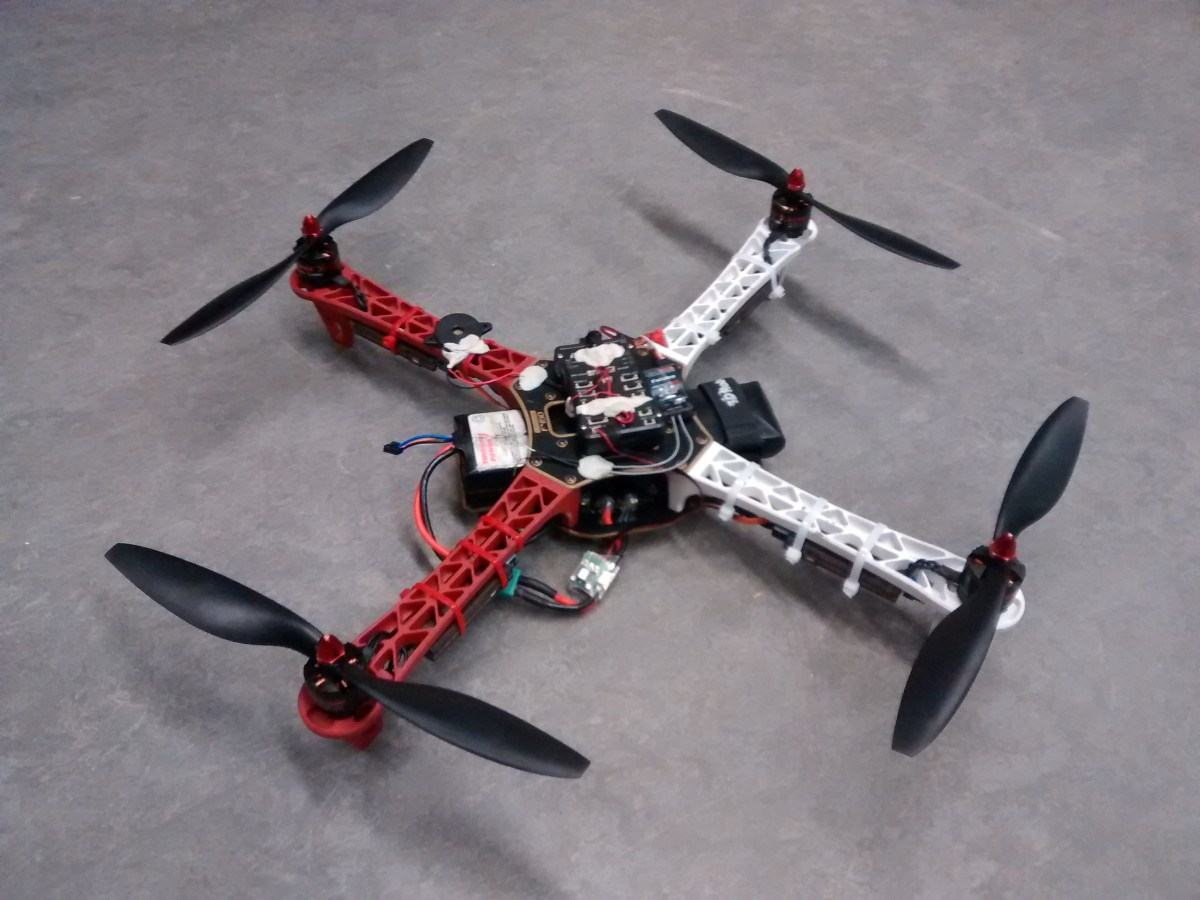
\includegraphics[width=0.8\linewidth]{images/quadrotor.jpg}
	\caption{DJI F450 with Pixhawk v1.5}
	\label{Quadrotor}
\end{figure}


\section{Results}
\begin{itemize}
	\item Results of the image stuff
	\begin{itemize}
		\item Plot of FPS vs distance
		\item Plot of true state vs mocap state?
	\end{itemize}
	
	\item PID/Control results 
	\begin{itemize}
		\item Plot XY for the controller loop
		\item Optimal PID settings
		\item How we got there
		\item Decent plot (V as a function of Z)
		\item Video?
	\end{itemize}
	
\end{itemize}
\subsection{PID and Controller Results}

So far the PID behaviours and gains have only been evaluated using a MOCAP system and tested only relative to a stationary target and these results are discussed herein. 




\section{Conclusion and Future Work}


\section{Proposed Future Work}
In the coming weeks, the PID controllers tested and developed using the MOCAP system will be tested using state estimates that are produced from the AprilTag library and the image preprocessing methods outlined in section \textbf{\textit{OUTLINE OF IMAGE PREPROCESSSING}}. 

One major issue highlighted in Ling \cite{Ling2014} is that due to the relatively long processing time of the AprilTags library, the estimated state obtained at a time $t$ does not actually represent the current state due to a time lag. This time lag as outlined in \cite{Ling2014} and defined in \ref{Detection Delay} must be accounted for when using the camera to estimate state. Currently our proposed method to measure this lag is to use the MOCAP system to provide a ground truth for the state from which we can estimate the estimated state.  

\begin{equation}
\label{Detection Delay}
    t_{\text{capture}} = t - \delta t_{\text{camera}} + \delta t_{\text{detection}}
\end{equation}

The next issue that will need to be address is the problem of the camera view. The dynamics of a quadrotor work in such a way that in order to move towards a goal point, the quadrotor must tilt away from the target which leads to problems with maintaining a view of the target when desired roll or pitch angles are greater than approximately 10 degress. This issue can either be addressed by mounting the camera at an angle or by adding a gimbals to the the quadrotor such that the gimbal will be sent commands by the onboard computer that will maintain a constant view of the target regardless of the commanded roll and pitch. 

Both of the above solutions have significant implementation questions that will have to be answered. If using the fixed camera angle, then the yaw of the qaudrotor will need to be controlled by a PID controller, similar to the the PID controllers to the roll and pitch. In the case of significant wind, the quadrotor will need to rotate itself such that the front of the quad is pointed into the wind during the final decent.

If a gimbal is used there are two issues that arise. First a new set of controllers that send roll, pitch and yaw commands to the gimbal such that the camera it is attached to maintains a centred view of the target platform must be developed. These controllers will likely be similar to the PID controllers developed above and so they are not considered to be terrible difficult to define are implement. The more difficult part of using a gimbal is related to resuming the gimbal state, which in cheaper gimbals do provide. All of the gimbals that have been researched as part of this project do not provide state feedback and so they are considered to be open loop. Therefore in order to use such a gimbal the user will need to assume the commanded gimbal position is equal to the true gimbal position, from which a transform between the quad rotor and the gimbal can be made.








\bibliography{report}{}
\bibliographystyle{ieeetr}






\end{document}
